\chapter{Building Logic Gates from Transistors}
\label{ch:cmos}

We have switches (Chapter~\ref{ch:mosfet}) and the algebra of 0s and 1s (Chapter~\ref{ch:binary}). This chapter joins them: it shows how NMOS and PMOS transistors are wired into logic gates, why the standard arrangement works so well, and what goes wrong when it is changed, including the swapped-inverter question from the assessment.

\section{The rule of complementary logic}

Every standard logic gate in a modern chip uses \term{static CMOS} (complementary MOS) design. Its output node is connected to two networks of transistors:

\begin{itemize}
  \item a \term{pull-up network} (PUN) of PMOS transistors, between the supply $\VDD$ and the output, which connects the output to 1;
  \item a \term{pull-down network} (PDN) of NMOS transistors, between the output and ground, which connects the output to 0.
\end{itemize}

The two networks are designed so that, for every combination of inputs, \emph{exactly one} of them conducts. The output is therefore always firmly connected to either the supply or ground, never to both and never to neither.

Why PMOS on top and NMOS on the bottom? Because of the strong and weak levels from Section~\ref{sec:weak1}: PMOS passes a strong 1 and NMOS passes a strong 0. Each transistor is placed where it is good.

\section{The CMOS inverter}

The simplest gate is the \term{inverter} (NOT gate): one PMOS and one NMOS, gates tied together as the input, drains tied together as the output (Figure~\ref{fig:inverter}).

\begin{figure}[h]
\centering
\begin{circuitikz}
  \draw (0,0) node[pmos](p){} (0,-2.2) node[nmos](n){};
  \draw (p.S) node[vdd]{$\VDD$};
  \draw (n.S) node[ground]{};
  \draw (p.D) -- (n.D);
  \draw (p.G) -- (n.G);
  \draw ($(p.G)!0.5!(n.G)$) to[short,-o] ++(-1,0) node[left]{In};
  \draw ($(p.D)!0.5!(n.D)$) to[short,*-o] ++(1.3,0) node[right]{Out};
\end{circuitikz}
\hspace{1.5cm}
\begin{circuitikz}
  \draw (0,0) node[not port](i){};
  \draw (i.in) -- ++(-0.4,0) node[left]{In};
  \draw (i.out) -- ++(0.4,0) node[right]{Out};
  \node at (0,-1.2) {logic symbol};
\end{circuitikz}
\caption{The CMOS inverter and its logic symbol.}
\label{fig:inverter}
\end{figure}

\begin{itemize}
  \item \textbf{Input = 0:} the PMOS is on (gate low) and the NMOS is off. The output connects to $\VDD$: output = 1.
  \item \textbf{Input = 1:} the NMOS is on and the PMOS is off. The output connects to ground: output = 0.
\end{itemize}

Three properties make this the ideal gate:
\begin{enumerate}
  \item \textbf{Full swing.} The output reaches exactly $\VDD$ and exactly 0\,V, because each transistor passes its strong level.
  \item \textbf{No static current.} In either steady state one transistor is off, so there is no path from supply to ground. An idle inverter burns only tiny leakage power.
  \item \textbf{Restoring.} The output is driven by the supply rails, not by the input, so a slightly noisy input still produces a clean output.
\end{enumerate}

\section{The voltage transfer characteristic}

What happens for inputs between 0 and $\VDD$? Plotting the output voltage against the input voltage gives the \term{voltage transfer characteristic} (VTC), Figure~\ref{fig:vtc}.

\begin{figure}[h]
\centering
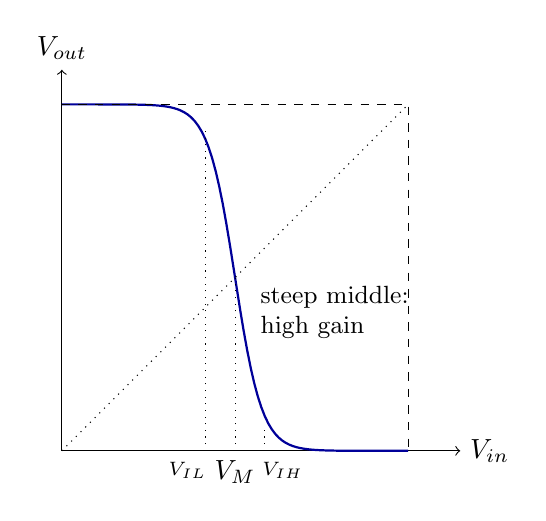
\begin{tikzpicture}[scale=1.1]
  \draw[->] (0,0) -- (4.6,0) node[right]{$V_{\text{in}}$};
  \draw[->] (0,0) -- (0,4.4) node[above]{$V_{\text{out}}$};
  \draw[thick,blue!60!black,domain=0:4,samples=100] plot (\x,{2*(1-tanh(3.2*(\x-2)))});
  \draw[dashed] (0,4) node[left]{$\VDD$} -- (4,4) -- (4,0) node[below]{$\VDD$};
  \draw[dotted] (0,0) -- (4,4);
  \draw[dotted] (2,0) node[below]{$V_M$} -- (2,2);
  \draw[dotted] (1.66,0) -- (1.66,3.75); \node[below] at (1.45,-0.02) {\scriptsize $V_{IL}$};
  \draw[dotted] (2.34,0) -- (2.34,0.25); \node[below] at (2.55,-0.02) {\scriptsize $V_{IH}$};
  \node[font=\small,align=left] at (3.15,1.6) {steep middle:\\high gain};
\end{tikzpicture}
\caption{Voltage transfer characteristic of an inverter. Where the curve crosses the diagonal, $V_{\text{in}} = V_{\text{out}} = V_M$.}
\label{fig:vtc}
\end{figure}

\begin{itemize}
  \item For low inputs the output stays near $\VDD$; for high inputs it stays near 0. In between, it drops steeply.
  \item In the steep middle both transistors are partly on. A current flows straight from supply to ground for the short time the input spends there (the short-circuit current, Chapter~\ref{ch:power}).
  \item The \term{switching threshold} $V_M$ is the input voltage at which $V_{\text{out}} = V_{\text{in}}$. With equally strong pull-up and pull-down (PMOS sized up to match the NMOS), $V_M = \VDD/2$. A stronger PMOS shifts $V_M$ higher, a stronger NMOS shifts it lower: the stronger side wins the tug-of-war, just like a voltage divider (Chapter~\ref{ch:electricity}).
  \item The steep middle means \emph{high gain}: the inverter acts as an amplifier there (Chapter~\ref{ch:analog}). This gain is what lets gates clean up noisy signals.
\end{itemize}

\paragraph{Noise margins.} Define four voltages:
\begin{itemize}
  \item $V_{OH}$, $V_{OL}$: the output levels a gate actually produces for 1 and 0;
  \item $V_{IH}$: the lowest input voltage guaranteed to be read as 1;
  \item $V_{IL}$: the highest input voltage guaranteed to be read as 0.
\end{itemize}
($V_{IL}$ and $V_{IH}$ are usually taken where the VTC's slope is $-1$.) The \term{noise margins} are how much noise a signal can pick up between one gate and the next and still be read correctly:
\[
  NM_H = V_{OH} - V_{IH}, \qquad NM_L = V_{IL} - V_{OL}.
\]
Larger is better. A CMOS inverter has $V_{OH} = \VDD$ and $V_{OL} = 0$, which gives it large noise margins.

\section{The swapped inverter}
\label{sec:swapped}

Now the assessment question. Take an inverter and swap the transistors: the NMOS now connects the output to $\VDD$, and the PMOS connects the output to ground (Figure~\ref{fig:swapped}). What does the circuit do?

\begin{figure}[h]
\centering
\begin{circuitikz}
  \draw (0,0) node[nmos](n){} (0,-2.4) node[pmos, xscale=1](p){};
  \draw (n.D) node[vdd]{$\VDD$};
  \draw (p.D) node[ground]{};
  \draw (n.S) -- (p.S);
  \draw (n.G) -- (p.G);
  \draw ($(n.G)!0.5!(p.G)$) to[short,-o] ++(-1,0) node[left]{In};
  \draw ($(n.S)!0.5!(p.S)$) to[short,*-o] ++(1.3,0) node[right]{Out};
  \node[right,font=\small] at (0.6,0.3) {NMOS on top};
  \node[right,font=\small] at (0.6,-2.7) {PMOS on bottom};
\end{circuitikz}
\caption{The ``swapped'' inverter: NMOS to the supply, PMOS to ground.}
\label{fig:swapped}
\end{figure}

Work through both inputs using the rules from Chapter~\ref{ch:mosfet}. Let $\VDD = 1.0$\,V, $\Vtn = 0.3$\,V and $|\Vtp| = 0.3$\,V.

\paragraph{Input = 1 ($\VDD$).} The top NMOS has its gate high, so it turns on and starts pulling the output \emph{up} toward $\VDD$. The bottom PMOS has its gate high, so it is off. But the NMOS is passing a 1, and NMOS passes a weak 1: the output is the NMOS's source, and the transistor turns off when the output reaches $\VDD - \Vtn = 0.7$\,V. The output settles at about 0.7\,V.

\paragraph{Input = 0.} The top NMOS is off. The bottom PMOS has its gate at 0, so it turns on and pulls the output \emph{down}. But PMOS passes a weak 0: the output is the PMOS's source, and the transistor turns off when the output falls to $|\Vtp| = 0.3$\,V. The output settles at about 0.3\,V.

\begin{center}
\begin{tabular}{ccc}
\toprule
Input & Normal inverter output & Swapped circuit output \\
\midrule
0 & $\VDD$ (strong 1) & $|\Vtp| = 0.3$\,V (weak 0) \\
1 & 0 (strong 0) & $\VDD - \Vtn = 0.7$\,V (weak 1) \\
\bottomrule
\end{tabular}
\end{center}

\begin{onoa}
The swapped circuit \textbf{no longer inverts}. It is a \textbf{non-inverting buffer with degraded output levels}: a high input gives a weak high ($\VDD - \Vtn$), and a low input gives a weak low ($|\Vtp|$). Each transistor acts as a \emph{source follower}: its output follows its gate, one threshold behind. The output swing is reduced, drive strength is weak (the transistors turn off as the output approaches its final value, so it gets there slowly), noise margins shrink, and the gain is less than 1, so the circuit cannot clean up noise. Chaining such stages makes it worse: in the simple model, a second stage driven by 0.7\,V can only reach $0.7 - 0.3 = 0.4$\,V, and the logic levels collapse.
\end{onoa}

The lesson generalizes: whenever a question puts NMOS in a pull-up position or PMOS in a pull-down position, expect a threshold-voltage drop on that level.

\section{NAND and NOR gates}

\subsection*{The two-input NAND}

A NAND gate's output is 0 only when both inputs are 1. So the pull-down network must conduct only when $A = 1$ \emph{and} $B = 1$: two NMOS transistors \textbf{in series} (current must pass through both, so both must be on). The pull-up must conduct whenever $A = 0$ \emph{or} $B = 0$: two PMOS transistors \textbf{in parallel} (either one can connect the output to $\VDD$). See Figure~\ref{fig:nandnor}, left.

\subsection*{The two-input NOR}

A NOR gate's output is 0 when $A = 1$ \emph{or} $B = 1$: two NMOS \textbf{in parallel}. Its output is 1 only when both inputs are 0: two PMOS \textbf{in series} (Figure~\ref{fig:nandnor}, right).

\begin{figure}[h]
\centering
\begin{circuitikz}[scale=0.9, transform shape]
  % NAND2
  \draw (0,0) node[pmos](pa){} (2,0) node[pmos](pb){};
  \draw (pa.S) -- (pb.S); \draw ($(pa.S)!0.5!(pb.S)$) node[vdd]{$\VDD$};
  \draw (pa.D) -- (pb.D);
  \draw (pb.D) -- ++(0,-0.6) coordinate(out);
  \draw (out) to[short,*-o] ++(1.2,0) node[right]{Out};
  \draw (out) -- ++(0,-0.3) coordinate(t);
  \draw (t) ++(0,-0.77) node[nmos,anchor=D](na){};
  \draw (na.S) ++(0,-0.77) node[nmos,anchor=D](nb){};
  \draw (t) -- (na.D);
  \draw (na.S) -- (nb.D);
  \draw (nb.S) node[ground]{};
  \node[left] at (pa.G) {A}; \node[left] at (pb.G) {B};
  \node[left] at (na.G) {A}; \node[left] at (nb.G) {B};
  \node at (1,-7.5) {NAND: PMOS parallel, NMOS series};
\end{circuitikz}
\hspace{1cm}
\begin{circuitikz}[scale=0.9, transform shape]
  % NOR2
  \draw (0,0) node[pmos](pa){};
  \draw (pa.S) node[vdd]{$\VDD$};
  \draw (pa.D) ++(0,-0.77) node[pmos,anchor=S](pb){};
  \draw (pa.D) -- (pb.S);
  \draw (pb.D) -- ++(0,-0.5) coordinate(out);
  \draw (out) to[short,*-o] ++(2.6,0) node[right]{Out};
  \draw (out) ++(0,-0.3) coordinate(t);
  \draw (out) -- (t);
  \draw (t) -- ++(2.0,0) coordinate(t2);
  \draw (t) ++(0,-0.77) node[nmos,anchor=D](na){};
  \draw (t2) ++(0,-0.77) node[nmos,anchor=D](nb){};
  \draw (t) -- (na.D); \draw (t2) -- (nb.D);
  \draw (na.S) -- (nb.S);
  \draw ($(na.S)!0.5!(nb.S)$) node[ground]{};
  \node[left] at (pa.G) {A}; \node[left] at (pb.G) {B};
  \node[left] at (na.G) {A}; \node[left] at (nb.G) {B};
  \node at (1.0,-7.5) {NOR: PMOS series, NMOS parallel};
\end{circuitikz}
\caption{Two-input NAND (left) and NOR (right). In each, the pull-up network is the \emph{dual} of the pull-down: series becomes parallel and parallel becomes series.}
\label{fig:nandnor}
\end{figure}

\begin{bigidea}
In the pull-down network, \textbf{series NMOS means AND} (all must be on) and \textbf{parallel NMOS means OR} (any can be on). The pull-up network is the \textbf{dual}: swap series and parallel, and use PMOS. This guarantees exactly one network conducts for every input combination.
\end{bigidea}

\section{Designing any gate}

The same recipe builds any inverting function:
\begin{enumerate}
  \item Write the function as $F = \nt{\text{something}}$, where ``something'' uses only ANDs and ORs of the inputs. That ``something'' is when the output should be 0.
  \item Build the pull-down network from it: AND becomes series NMOS, OR becomes parallel NMOS.
  \item Build the pull-up network as the dual: swap series and parallel, use PMOS, same inputs.
\end{enumerate}

\begin{worked}{an AND-OR-INVERT gate}
Build $F = \nt{AB + C}$ (called AOI21: AND-OR-INVERT with a 2-input AND and a 1-input term).

Pull-down conducts when $AB + C = 1$: NMOS $A$ in series with NMOS $B$, and that pair in parallel with NMOS $C$.

Pull-up is the dual: PMOS $A$ in parallel with PMOS $B$, and that pair in series with PMOS $C$.

Total: 6 transistors. Building the same function from separate AND, OR and NOT gates would take 12 or more, and be slower. Compound gates like AOI and OAI (OR-AND-INVERT) are common for this reason.
\end{worked}

\paragraph{Why static CMOS gates always invert.} In a single stage, turning an input \emph{on} (to 1) can only turn NMOS transistors on, which can only pull the output \emph{down}. So a rising input can only cause a falling output. A non-inverting function needs two stages: AND is a NAND followed by an inverter, OR is a NOR followed by an inverter.

\begin{center}
\begin{tabular}{lc}
\toprule
Gate & Transistors (static CMOS) \\
\midrule
Inverter & 2 \\
NAND2, NOR2 & 4 \\
NAND3, NOR3 & 6 \\
AND2, OR2 (gate + inverter) & 6 \\
AOI21, OAI21 & 6 \\
XOR2 (straightforward static design) & 12 \\
\bottomrule
\end{tabular}
\end{center}
An $n$-input static CMOS gate uses $2n$ transistors: one NMOS and one PMOS per input.

\section{Why NAND is preferred over NOR}

NAND and NOR are both universal (Chapter~\ref{ch:comb}), but designers strongly prefer NAND. The reason is mobility. Transistors in series are slower, because their resistances add (Chapter~\ref{ch:electricity}). A NAND puts its series stack in the NMOS, which is the fast device. A NOR puts its series stack in the PMOS, which is already about two to three times slower. To compensate, the series PMOS in a NOR must be made very wide, which costs area and adds input capacitance.

Sizing for the same strength as a reference inverter (NMOS width 1, PMOS width 2, assuming $\mu_n = 2\mu_p$):
\begin{center}
\begin{tabular}{lll}
\toprule
Gate & Each NMOS & Each PMOS \\
\midrule
Inverter & 1 & 2 \\
NAND2 & 2 (two in series) & 2 (in parallel) \\
NOR2 & 1 (in parallel) & 4 (two in series) \\
\bottomrule
\end{tabular}
\end{center}
Two transistors in series act like one with twice the resistance, so each must be twice as wide to keep the same total strength. The NOR's PMOS pair ends up four times the NMOS width.

\paragraph{Fan-in limits.} The more inputs a gate has, the taller its series stack. Tall stacks are slow, both because resistances add and because the upper transistors suffer the body effect (Chapter~\ref{ch:mosfet}). Gates are usually limited to about four inputs; wider functions are built as trees of smaller gates.

\section{Pass transistors and transmission gates}

Instead of connecting outputs to the supply rails, a \term{pass transistor} simply passes an input signal through. A single NMOS pass transistor is small, but it passes a weak 1. The fix is the \term{transmission gate} (TG): an NMOS and a PMOS in parallel, controlled by opposite signals (Figure~\ref{fig:tg}). When the control is on, both conduct: the NMOS carries the 0s well and the PMOS carries the 1s well, so the TG passes \emph{both} levels at full strength.

\begin{figure}[h]
\centering
\begin{circuitikz}
  \draw (0,0) node[nmos, rotate=90](n){};
  \draw (0,1.8) node[pmos, rotate=-90](p){};
  \draw (n.D) -- (p.D); \draw (n.S) -- (p.S);
  \draw ($(n.D)!0.5!(p.D)$) to[short,*-o] ++(-1,0) node[left]{In};
  \draw ($(n.S)!0.5!(p.S)$) to[short,*-o] ++(1,0) node[right]{Out};
  \draw (n.G) -- ++(0,-0.4) node[below]{$S$};
  \draw (p.G) -- ++(0,0.4) node[above]{$\nt{S}$};
\end{circuitikz}
\caption{A transmission gate: when $S = 1$, both transistors conduct and the input passes to the output at full strength.}
\label{fig:tg}
\end{figure}

Transmission gates make compact multiplexers (two TGs and an inverter make a 2:1 mux), XOR gates, and the latches inside flip-flops (Chapter~\ref{ch:latch}). Their drawback is that they do not restore signal levels or add drive; a long chain of TGs gets slow and must be broken up with buffers.

\section{Tristate buffers}

Sometimes several circuits must share one wire, such as a bus. Only one may drive it at a time; the others must disconnect. A \term{tristate buffer} has an enable input. When enabled, it drives its input value (0 or 1) onto the output. When disabled, both its pull-up and pull-down are off and the output is disconnected, a third state called \term{high impedance} or \term{Z}. If two enabled drivers fight over one wire (one driving 1, the other 0), the result is \term{contention}: a large current flows between them and the wire sits at an undefined middle voltage.

\section{Other logic styles}

\paragraph{Dynamic logic.} A dynamic gate replaces the pull-up network with a single clocked PMOS. In the \emph{precharge} phase (clock low), it charges the output high. In the \emph{evaluate} phase (clock high), a clocked NMOS ``foot'' turns on and the NMOS pull-down network discharges the output if the logic function says so. Dynamic gates use fewer transistors and are fast, but the precharged output is held only by capacitance, so it can leak away, be disturbed by noise, or lose charge to internal nodes (\term{charge sharing}). They also need a clock and burn more power. \term{Domino logic} adds an inverter after each dynamic gate so that cascaded gates work correctly.

\paragraph{Ratioed logic (pseudo-NMOS).} Replace the pull-up network with a single PMOS that is always on, acting like a resistor. The pull-down network must overpower it to make a 0. It saves transistors, but the output low is set by a tug-of-war (a voltage divider), so it never reaches exactly 0\,V, and current flows from supply to ground continuously whenever the output is low: static power.

\section{Summary}

\begin{itemize}
  \item Static CMOS: PMOS pull-up network to $\VDD$, NMOS pull-down network to ground, exactly one conducting.
  \item The inverter has full swing, no static current, high gain and restores clean levels.
  \item VTC: $V_M = \VDD/2$ when balanced; the stronger device pulls $V_M$ toward its side. Noise margins $NM_H = V_{OH} - V_{IH}$, $NM_L = V_{IL} - V_{OL}$.
  \item Swapped inverter (NMOS up, PMOS down): non-inverting buffer with weak levels, $\VDD - \Vtn$ and $|\Vtp|$; gain below 1; degrades when chained.
  \item Pull-down: series NMOS = AND, parallel = OR. Pull-up is the dual.
  \item Single-stage static CMOS gates are inverting. $n$ inputs need $2n$ transistors.
  \item NAND beats NOR because NOR stacks slow PMOS in series.
  \item Transmission gates pass both levels strongly. Tristate outputs can disconnect (Z).
  \item Dynamic logic is fast but fragile; pseudo-NMOS burns static power.
\end{itemize}

\section{Exercises}

\begin{enumerate}
  \item In a CMOS inverter with input 0, which transistor is on, and what is the output?
  \item How much static current does an ideal CMOS inverter draw when its input is steady?
  \item The PMOS in an inverter is made much stronger than the NMOS. Does $V_M$ move up or down?
  \item A swapped inverter has $\VDD = 1.2$\,V, $\Vtn = 0.4$\,V, $|\Vtp| = 0.35$\,V. What are the outputs for input 1 and input 0? Is it an inverter?
  \item How many transistors are in a static CMOS NOR3? In an AND2?
  \item Design the pull-down and pull-up networks for $F = \nt{(A + B)\,C}$ (an OAI21 gate).
  \item Why are NAND gates generally preferred over NOR gates?
  \item Assuming $\mu_n = 2\mu_p$ and a reference inverter with NMOS width 1, size a NOR2 for equal pull-up and pull-down strength.
  \item Why does a transmission gate pass both 0 and 1 at full strength?
  \item Give one advantage and one disadvantage of dynamic logic.
  \item A gate has $V_{OH} = 1.0$\,V, $V_{OL} = 0.05$\,V, $V_{IH} = 0.6$\,V and $V_{IL} = 0.4$\,V. Find both noise margins.
  \item True or false: a single static CMOS stage can implement AND.
\end{enumerate}

\subsection*{Answers}
\begin{enumerate}
  \item The PMOS is on (its gate is low), connecting the output to $\VDD$: output = 1.
  \item Essentially none; only leakage, because one transistor is always off.
  \item Up: the stronger pull-up wins the tug-of-war until the input is higher.
  \item Input 1: $1.2 - 0.4 = 0.8$\,V. Input 0: 0.35\,V. It does not invert; it is a weak, non-inverting buffer.
  \item NOR3: 6. AND2: 6 (a NAND2 plus an inverter).
  \item Output is 0 when $(A + B)C = 1$. Pull-down: NMOS $A$ parallel with NMOS $B$, that pair in series with NMOS $C$. Pull-up (dual): PMOS $A$ in series with PMOS $B$, that pair in parallel with PMOS $C$.
  \item NOR puts the slow PMOS transistors in series, making the pull-up slow or requiring very wide PMOS devices. NAND puts the fast NMOS in series and the PMOS in parallel.
  \item Each NMOS width 1 (parallel), each PMOS width 4 (two in series, each needs twice the reference PMOS width of 2).
  \item Its NMOS passes a strong 0 and its PMOS passes a strong 1; with both on in parallel, whichever level is being passed has a strong path.
  \item Advantage: fewer transistors and faster. Disadvantage: the output is held only by charge, so it is sensitive to leakage, noise and charge sharing; it also needs a clock and uses more power.
  \item $NM_H = 1.0 - 0.6 = 0.4$\,V. $NM_L = 0.4 - 0.05 = 0.35$\,V.
  \item False. A single static CMOS stage is always inverting; AND needs NAND plus an inverter.
\end{enumerate}
